\section{Introduction, general remarks about the grid point
method}\label{Chapter1}

In this chapter, following a short historical introduction on the
development and use of numerical methods in atmospheric models, methods
available for numerical solution of the differential equations governing
the atmosphere will be briefly reviewed. Then, basic elements of the
finite difference method for solving these equations will be introduced.
Finally, the concept of stability of finite difference equations, and
methods for testing the stability of such equations, will be discussed
at some length.

\subsection{\texorpdfstring{\textbf{Historical
introduction}}{Historical introduction}}\label{historical-introduction}

It is considered that Wilhelm Bjerknes (1904) was the first to point out
that the future state of the atmosphere can in principle be obtained by
an integration of differential equations which govern the behaviour of
the atmosphere, using as initial values fields describing an observed
state of the atmosphere. Such an integration performed using numerical
methods is called numerical weather prediction. When, however, a
numerical integration is performed starting from fictitious initial
fields, it is called numerical simulation.

A first practical attempt at a numerical weather prediction was made by
Richardson. After very tedious and time-consuming computations, carried
out mostly during the First World War, Richardson obtained a totally
unacceptable result. Despite this, he described his method and results
in a book (Richardson, 1922), and this is today one of the most famous
in meteorology.

The wrong result obtained by Richardson, and his estimate that 64,000
men are necessary to advance the calculations as fast as the weather
itself is advancing, left some doubt as to whether the method would be
of practical use. A number of developments that followed, however,
improved the situation. Courant, Friedrichs and Lewy (1928) found that
space and time increments in integrations of this type have to meet a
certain stability criterion. Mainly due to the work of Rossby in the
late 1930\textquotesingle s, it became understood that even a rather
simple equation, that describing the conservation of absolute vorticity
following the motion of air particles, suffices for an approximate
description of large-scale motions of the atmosphere. Finally, in 1945,
the first electronic computer ENIAC (Electronic Numerical Integrator and
Computer) was constructed. The absolute vorticity conservation equation,
and this first electronic computer, were used by Charney, Fjortoft and
von Neumann in the late 1940\textquotesingle s for the first successful
numerical forecast (Charney et al., 1950).

Much faster computers, and improved understanding of computational
problems, now also enable long-term integrations of the basic primitive
equations. It is generally considered that integration of the primitive
equations enables easier incorporation of various physical processes
than the integration of modified equations, that is, integration of the
divergence and vorticity equations. Thus, it is mostly the primitive
equations that are used today for practical numerical forecasting by
meteorological services. Charts obtained by numerical forecasting are
used by synopticians in these services as the principal basis for
decisions on forecasts issued for public use.

A number of research groups have been actively engaged for more than a
decade in development of models for the numerical simulation of the
general circulation of the atmosphere. In such simulations starting from
a fictitious initial state, e.g. an isothermal and motionless
atmosphere, is often considered to be an advantage for the experiments.
It enables a test of the ability of the computational and physical
schemes of the model to simulate an atmosphere with statistical
properties similar to those of the real atmosphere, with no, or not
much, prior information on these properties.

Numerical models are also very frequently developed for studies of some
smaller-scale atmospheric phenomena. Foremost among these are studies of
the cumulus convection problem, and simulation of processes within the
planetary boundary layer. In this text, however, we shall primarily have
in mind the application of numerical methods to prediction and
simulation of large-scale atmospheric motions.

\subsection{\texorpdfstring{\textbf{Methods for the numerical solution
of the equations of
motion}}{Methods for the numerical solution of the equations of motion}}\label{methods-for-the-numerical-solution-of-the-equations-of-motion}

Numerical solution of the equations of motion today in most cases is
performed using the \emph{grid point method}. In this method a set of
points is introduced in the region of interest and dependent variables
are initially defined and subsequently computed at these points. This
set of points is called the \emph{grid}. The words \emph{mesh or
lattice} are also used. It is necessary to have the grid points at fixed
locations in the horizontal. This means that, according to the Eulerian
system of equations, space and time coordinates are chosen as
independent variables.

A number of attempts have been made to develop atmospheric models using
an approach which is at least partly Lagrangian. Serious difficulties
are encountered when a straightforward numerical integration of the
Lagrangian system of equations is undertaken. However, it is possible to
construct methods with some Lagrangianproperties ; for example, to have
some or all of the computation points moving with the fluid. In
hydrodynamics a number of such methods have proved to be very useful,
especially for some problems which are not amenable to treatment by a
strictly Eulerian technique (e.g. Harlow and Amsden, 1971). However, in
meteorology the performance of Lagrangian or semi-Lagrangian models
that have so far been developed has not been quite satisfactory. A
discussion of one way of constructing a Lagrangian model, and a review
of earlier attempts, can be found in a paper by Mesinger (1971).

Another possible approach is to express the spatial dependence of the
variables in terms of a series of orthogonal functions, and then
substitute this into the governing equations. In this way the equations
reduce to a set of ordinary differential equations, so that the
coefficients of the series can be computed as functions of time. This is
the \emph{spectral method} of solving the governing equations. Until
relatively recently it was considered that in effiÂciency the spectral
method could not be competitive with the grid point method. But the use
of the fast Fourier transform has completely changed the situation and
investigation of spectral methods is now the subject of intensive
research.

In the following we shall consider the technique of using the grid point
method, and the problems associated with it, using grid of computation
points fixed in space. This is the most direct way of solving the
equations of motion numerically. Furthermore, knowledge of this method
is necessary for the investigation and understanding of the relative
merits of other alternatives mentioned in this section.

\subsection{\texorpdfstring{\textbf{Basic elements of the grid point
method}}{Basic elements of the grid point method}}\label{basic-elements-of-the-grid-point-method}

With the grid point method, the most common way of solving the governing
equations is to find approximate expressions for derivatives appearing
in the equations. These approximate expressions are defined using only
values of the dependent variables at the grid points, and at discrete
time intervals. Thus, they are formed using differences of dependent
variables over finite space and time intervals; for that reason this
approach is called the \emph{finite difference method}. The
approximations for derivatives are then used to construct a system of
algebraic equations that approximates the governing partial differential
equations. This algebraic system is considered valid at each of the
interior grid points of the computation region. For the initial time and
at space boundary points, additional constraints or equations are
defined that approximate the initial and boundary conditions as
required by the physics of the problem. The set of algebraic equations
obtained in this way is then solved, usually using an electronic
computer, by a suitable step-wise procedure.

We shall now consider some basic elements of the finite difference
method. For simplicity, we start by considering a function of one
independent variable

\[u = u(x)\]

The function \emph{u} is a solution to a differential equation that we
are interested in. We want to find an approximation to this solution in
a bounded region R of the independent variable, having a length
\emph{L}. The simplest way of introducing a set of grid points is to
require that they divide the region R into an integer number of
intervals of equal length \(\Delta x\). This length \(\Delta x\) is
called the \emph{grid interval}, or \emph{grid length}. Let us denote
the number of grid intervals by \emph{J}. It is convenient to locate the
origin of the \emph{x} axis at the left-hand end of the region R. Thus,
we are looking for approximations to \(u (\mathcal{x)}\) at discrete
points \(\mathcal{x = j}\Delta\mathcal{x, }\) where \emph{j} takes
integer values 0,1,2,... \emph{J}. These approximate values we shall
denote by

\[u_j = u_j(j \Delta x)\]

Thus, we are interested in finding \emph{J} + 1 values \(u_ j\)

Knowledge of a discrete set of values \(u_j\), even if the
approximations were perfect, offers, obviously, less information than
knowledge of the function \emph{u} (\emph{x}). Let us briefly consider
the situation in that respect. We shall very often find it convenient to
think of the function \emph{u} (\emph{x}) as being formed by a sum of
its Fourier components, that is

\[u( x ) = \frac{a_{0}}{2} + \sum_{n \geq 1}(\left[  a_{n}  \cos\left(2\pi n \frac{x}{L}\right)
+ b_{n}   \sin\left(2\pi n \frac{x}{L} \right))\right]\]

Now, the available \emph{J} + 1 values \(u_j\) do not enable the
computation of all of the coefficients \(a_{n}b_{n}\); rather, they can
be used to compute only \emph{J} + 1 different coefficients. A natural
choice is to assume that the \emph{J} + 1 values \(u_j\) define the near
value \(a_{0}\) and as many as possible of the coefficients of the
Fourier components at the long wave length end of the series, that is,
coefficients for \emph{n} = 1,2,3,..., \emph{J/} 2. Of these components,
the one with the shortest wavelength will have n=J/2, with the wave
length

\[\frac{L}{n} =  \frac{2L}{j} =  \frac{2L}{\frac{L}{\Delta\mathcal{x}}} = 2\Delta\mathcal{x}\]

Having made that choice, we can say that with values \(u_{j}\) at
discrete points \(\mathcal{x =}j\Delta\mathcal{x}\) it is not possible
to resolve waves with wave length shorter than $2 \Delta x$.

Now let us consider the differences between values u\} that will be used
to construct approximations to derivatives. These differences are
called \emph{finite differences}. They can be calculated over one or
more of the intervals Ax. Depending on the relation of the points from
which the values are taken to the point where the derivative is
required, they can be \emph{centered or uncentered}. An un-centered
difference is, for example, the \emph{forward} difference

\[\Delta u_{\text{i }} = u_{j + 1}  - u_{j}\]

More often centered (or \emph{central}) differences are used, such as

\[\text{δu}_{j + \frac{1}{2}} =  u_{i + 1} -  u_{j}\]

In a centered difference the difference is between values symmetrical
about the point where the difference is being calculated.

One way to construct an approximation to a differential equation is to
simply replace the derivatives by appropriate \emph{finite difference
quotients}. For example, for the first derivative one can use the
approximation

    {\[\left( \frac{d u}{d x } \right)_j \to \frac{u_{j + 1} - u_{j}}{\Delta x}\]}

The finite difference quotient here is, of course, only one of many
possible approximations to the first derivative at point j.

If a finite difference quotient, or a more complex expression, is to be
used as an approximation to a derivative, it is required, above all,
that this approximation be consistent. This means that the approximation
should approach the derivative when the grid interval approaches zero.
The quotient \texttt{3.1} , obviously, has that property.

Important information is obatined when the true solution
\(u (j\Delta x)\) is substituted into an approximation to the derivative
in place of the grid point values \(u_{j}\), and \(u(j\Delta x)\) is
expanded in a Taylor series about the central point. For the quotient
\texttt{3.1} this procedure gives

\[\frac{u_{j+1} - u_j}{\Delta x} \to \left( \frac{d u}{d x} \right)_j +
\frac{1}{2} \left( \frac{d^2 u}{dx^2} \right)_j \Delta x +
\frac{1}{6} \left( \frac{d^3 u}{dx^3} \right)_j
( \Delta x )^2 + \ldots\]

The difference between this expression and the derivative

\[\left( \frac{\text{du}}{\text{dx}} \right)_{j}\]

being approximated. In this case

\[\varepsilon = \frac{1}{2}\left( \frac{d^{2}u}{\text{dx}^{2}} \right)\Delta x + \frac{1}{6}\left( \frac{\text{du}^{3}}{\text{dx}^{3}} \right)_{j}\]

is called the truncation error of the approximation to the derivative.
These are terms that were "truncated off" to form the approximation. The
truncation error gives a measure of how accurately the difference
quotient approximates the derivative for small values of $\Delta x$.

The usual measure of this is the order of accuracy of an approximation.
This is the lowest power of Ax that appears in the truncation error.
Thus, approximation (3.1) is of the first order of accuracy. We can
write

\[\varepsilon = 0(\Delta x)\]

For an approximation to the derivative to be consistent it must,
obviously, be at least first order accurate.

\subsection{\texorpdfstring{\textbf{Finite difference
schemes}}{Finite difference schemes}}\label{finite-difference-schemes}

The algebraic equation obtained when derivatives in a differential
equation are replaced by appropriate finite difference approximations is
called a finite difference approximation to that differential equation,
or a finite difference scheme. In this section we shall introduce the
concepts of consistency, truncation error, and accuracy, for a finite
difference scheme.

As an example, we shall use the linear advection equation

    {\[\frac{\partial u}{\partial t} +c\frac{\partial u}{\partial x } = 0; u =u(x,t)\]}

\emph{c} is a positive constant.

It describes advection of the variable u at a constant velocity c in the
direction of the x axis. The solution to this simple equation can, of
course, also be obtained by an analytic method. It will be useful to
obtain the analytic solution first, in order to investigate properties
of numerical solutions by comparing them against known properties of the
true solution.

It is convenient to this end to change from variables \emph{x}, \emph{t}
to variables, \(\xi,\) \emph{t} with the substitution \(\xi = x - ct\).

Using the notation

\[u^{(x,t)} = U (\xi, t)\]

we obtain

\[\frac{\partial u}{\partial t} = \frac{\partial U}{\partial\xi}\frac{\partial\xi}{\partial y} +
\frac{\partial U}{\partial t}\frac{\partial t}{\partial t} =-c\frac{\partial U}{\partial\xi}+
\frac{\partial U}{\partial t}\]

\[\frac{\partial u}{\partial x} =\frac{\partial U}{\partial\xi}\frac{\partial\xi}{\partial X}
+ \frac{\partial U}{\partial t}\frac{\partial t}{\partial x}\frac{\partial U}{\partial\xi}\]

Substitution of these expressions into \texttt{g4.1} gives

\[\frac{\partial}{\partial t}U(\xi,t) = 0\]

Thus, it is seen that U cannot be a function of t, but can be an
arbitrary function of \(\xi\). A solution of \texttt{g4.1} is,
therefore,

    {\[u = f(x - ct)\]}

where \emph{f} is an arbitrary function. This, we see, is the general
solution of the advection equation \texttt{g4.1}, since it can satisfy
an arbitrary initial condition

    {\[u(x,0) = F(x)\]}

Thus,

    {\[u = F \left( x - ct \right)\]}

is the solution of \texttt{g4.1} satisfying the initial condition
\texttt{g4.3}.

For a physical interpretation, it is often convenient to consider the
solution in the \emph{x, t} plane. In the present case, we see that the
solution takes constant values along the straight lines

\[x - ct = const.\]

These lines are the \emph{characteristics} of the advection equation ;
one of them is shown in \texttt{figg:1}. We can say that the solution
propagates along the characteristics.

\begin{figure}
    \centering
    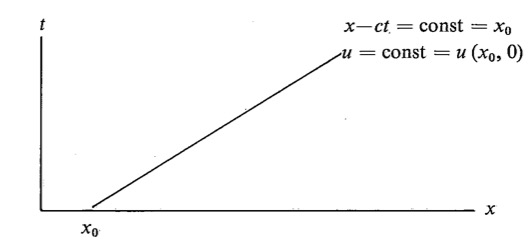
\includegraphics[width=0.8\linewidth,height=\textheight,width = .7 \textwidth]{figs/NM/pic1.jpg}
    \caption{One of the characteristics of the linear advection equation
    \texttt{g4.1}}
\end{figure}

Let us now construct a scheme for finding an approximate solution to
\texttt{g4.1} using the grid point method.

We are now looking only for an approximate solution at the discrete
points in the \((x,t)\) plane formed by the grid shown in Fig.
\texttt{figg:1}. The approximate solution at a point
\(\left( j\Delta x, n\Delta t) \right)\) is denoted by \(u_{j}^{n}\).

\begin{figure}
    \centering
    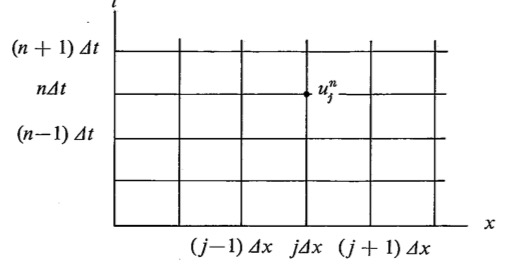
\includegraphics[width = .7 \textwidth]{figs/NM/pic2.jpg}
    \caption{} \label{fig:}
\end{figure}

The behaviour of the true solution, which propagates along
characteristics in the (x,t) plane, suggests constructing the
approximate equation by replacing the time derivative by a forward
difference quotient, and the space derivative by a backward difference
quotient. In this way we obtain the scheme

    {\[\frac{u_{j}^{n + 1} - u_{j}^{n}}{\Delta t} + c\frac{u_j^n - u_{j - 1}^n}{\Delta x} = 0\]}

This scheme could be called a forward and upstream scheme, the latter
word indicating the position of the point \(j - 1\) relative to the
advection velocity. It is, of course, only one of many possible
consistent finite difference schemes for the differential equation.
There are many schemes which approach the differential equation when the
increments \(\Delta x,\Delta t\) approach zero.

Since for small values of \(\Delta x,\Delta t\) a finite difference
equation approximates the corresponding differential equation, we can
expect that its solution will be an approximation to the solution of
that equation. We shall call solutions given by finite difference
schemes numerical solutions. There are, of course, both approximate and
numerical solutions obtained by other methods which will not be
considered in this publication. It is most convenient to study the
properties of numerical solutions when they can be compared with known
solutions of the original differential equation, which we shall refer to
as true solutions. The difference between the numerical and the true
solution

    {\[u_{j}^{n}-u ( j\Delta x,n\Delta t )\]}

is the error of the numerical solution.

For obvious reasons, we cannot often expect to know the error of the
numerical solution. However, we can always find a measure of the
accuracy of the scheme by substituting the true solution
\(u \left( j\Delta x,n\Delta t \right)\) of the equation, into the
numerical scheme. Since the true solution will not satisfy the numerical
equations exactly, we will have to add an additional term to keep the
equation valid. Let us denote this term by \(\varepsilon\) . For
example, in the case of scheme \texttt{g4.5} this procedure gives

    {\[\frac{u\left( j\Delta x,( n + 1 )\Delta t \right)
    - u\left( j\Delta x,\Delta\text{nt} \right)}{\Delta t}
+ c\frac{u\left( j\Delta x,n\Delta t \right)
- u\left( \left( j - 1 \right)\Delta x,\Delta t \right)}{\Delta x} = \varepsilon\]}

The term e we shall call the truncation error of the finite difference
scheme. It shows how closely the true solution satisfies the equation of
the scheme, and, thus, gives a measure of the accuracy of the scheme.

We can obtain a more useful form for the expression for the truncation
error by performing a Taylor series expansion of the true solution about
the central space and time point. Using the original differential
equation to eliminate the leading term we obtain the truncation error
\texttt{g4.7} as

    {\[\varepsilon = \frac{1}{2}\frac{\partial^{2u}}{{\partial t}^{2}}\Delta t
+ \frac{1}{6}\frac{\partial^{3}u}{{\partial t}^{3}}\left( \Delta t \right)^{2} +\ldots-
c(\frac{1}{2}\frac{\partial^{2}u}{{\partial x}^{2}}\Delta x -
\frac{1}{6}\frac{\partial^{3}u}{{\partial t}^{3}}\left( \Delta x \right)^{2}
+\ldots )\]}

As before, these are the terms that were "truncated off" to make the
differential equation reduce to our finite difference scheme.

In the same way as for an approximation to the derivative, the order of
accuracy of a finite difference scheme is the lowest power of Ax and At
that appears in the truncation error. Thus, scheme \texttt{g4.5} is
first order accurate. We can write

\[\varepsilon = O \left( \Delta t \right) + O\left( \Delta x \right)\]

or

\[\varepsilon = O \left( \Delta x,\Delta t \right).\]

It is useful to make a distinction between orders of accuracy in space
and in time, especially when the lowest powers of \(\Delta x\) and
\(\Delta t\) are not the same. As before, a necessary condition for
consistency of a scheme is that it be at least of the first order of
accuracy.

\subsection{\texorpdfstring{\textbf{Convergence}}{Convergence}}\label{Section1.5}

The truncation error of a consistent scheme can be made arbitrarily
small by a sufficient reduction of the increments \(\Delta x\) and
\(\Delta t\). Unfortunately, we cannot be sure that this will also
result in a reduction of the error of the numerical solution. For that
reason, we return to consideration of the error

\[u_j^n-u\left( j\Delta x,n\Delta t \right).\]

Following Richtmyer and Morton (1967) we ask two questions:

(a) What is the behavior of the error
\(u_{j}^{n} - u\left( j\Delta x,n\Delta t \right)\) when, for a fixed
total time \(n \Delta t\) the increments \(\Delta x , \Delta t\)
approach zero ?

(b) What is the behavior of the error
\(u_{j}^{n} - u\left( j\Delta x,n\Delta t \right)\) when, for fixed
values of \(\Delta x, \Delta t\), the number of time steps \emph{n}
increases?

The answer to the first of these questions depends on the convergence of
the numerical solution : if the error approaches zero as the grid is
refined ( as \(\Delta x, \Delta t \rightarrow 0\) ) the solution is
called convergent. If a scheme gives a convergent solution for any
initial conditions, then the scheme also is called convergent.

Consistency of a scheme does not guarantee convergence. We shall
illustrate this by a simple example. We still consider the scheme
\texttt{g4.5}; its truncation error \texttt{g4.8} approaches zero as the
grid is refined, and, therefore, this is a consistent scheme. But
consider the numerical solution, when the grid lines and
characteristics are as shown in \texttt{figg:3}. The characteristic
passing through the grid point taken as the origin in this example
passes through another grid point, A, denoted by a square. Thus, the
true solution at A, is equal to the initial value at the origin. However
the numerical solution given by \texttt{g4.5} A is computed using the
values at points denoted by circles. The shaded domain, including all of
these points, is called the domain of dependence of the numerical
scheme. The grid point at the origin is outside that domain, and, thus,
cannot affect the numerical solution at \(A_0\). Therefore, the error
can be arbitrarily great. If the space and time steps were reduced by
the same relative amount, say to one half of their values in the figure,
the domain of dependence would still remain the same, and this situation
would not change. Thus, as long as the ratio of the steps \(\Delta x\)
and \(\Delta t\) remains the same, refinement of the grid cannot bring
about a reduction in the error of the numerical solution.

\[x - ct = const\]

\begin{figure}
    \centering
    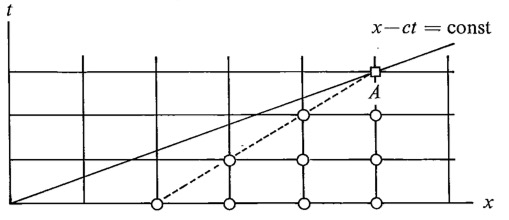
\includegraphics[width = .7 \textwidth]{figs/NM/pic3.jpg}
    \caption{} \label{fig:}
\end{figure}

A necessary condition for convergence of a scheme is, obviously, that
the characteristic defining the true solution at a grid point is inside
the domain of dependence of the numerical solution at that point. In our
example, this will happen when the slope of the characteristics is
greater than the slope of the dashed line bounding the domain of
dependence, that is, when

    {\[c\Delta t \leq \Delta x\]}

Thus, this is a necessary condition for convergence of \texttt{g4.5}.

\subsection{\texorpdfstring{\textbf{Stability}}{Stability}}\label{stability}

The answer to the second question raised at the beginning of the
Section \texttt{Section1.5} depends on the stability of the numerical
solution. A rigorous definition of stability employs the concepts of
functional analysis, and refers to the boundedness of the numerical
solution only (e.g. Richt-myer and Morton, 1967). The difficulties in
defining stability are caused by the fact that the true solution, in
general, does not have to be bounded. However, when we know that the
true solution is bounded, as in the equations we are interested in here,
we can use a definition referring to the boundedness of the error
\(u_{j}^{n} - u\left( j\Delta x,n\Delta t \right)\text{. }\) We sat that
a solution \(u_{j}^{n}\) is stable if this error remains bounded as n
increases, for fixed values of \(\Delta x,\Delta t.\) As before, we say
that a finite difference scheme is stable if it gives a stable solution
for any initial conditions.

Stability of a scheme is a property of great practical significance.
There are consistent schemes, of a high order of accuracy, that still
give solutions diverging unacceptably fast from the true solution. Thus,
conditions for stability, if any, should be known. There are three
methods that can be used to investigate the stability of a scheme, and
we shall give an example of each of these methods. We shall do this by
considering again the forward and upstream scheme \texttt{g4.5}).

\emph{Direct method}. Since we know that the true solution is bounded,
it suffices to test the boundedness of the numerical solution. The
scheme \texttt{g4.5} can be written as

    {\[u_{j}^{n + 1} = \left( 1 - \mu \right)u_{j}^{n}+ \mu u_{j - 1}^{n}\]}

where

\[\mu \equiv C\Delta t/\Delta x.\]

If \(1 - \mu \geq 0,\) which happens to be also the necessary condition
for convergence, we will have

    {\[\left| u_{j}^{n + 1} \right| \leq \left( 1 - \mu \right)\left| u_{j}^{n} \right| + \mu\left| u_{j - 1}^{n} \right|.\]}

We can apply this at the point where at time level \emph{n + 1} ,
\(\left| u_{j}^{n + 1} \right|\) is a maximum,
\({Max}_{(j)} \left | u_{j}^{n + 1} \right|\). The right side of
\texttt{g6.2} can only be increased by replacing
\(\left| u_{j}^{n} \right|\) and \(\left| u_{j-1}^{n} \right|\) by the
maximum value at level n, \({Max}_{(j)} \left| u_{j}^{n} \right|\).The
two terms on the right side can then be added, and we obtain

\[{Max}_{(j)} \left| u_{j}^{n + 1} \right| \leq {Max}_{(j)}\left| u_{j}^{n} \right|\]

This proves the boundedness of the numerical solution. Hence,
\(1 - \mu \geq 0\) is seen to be a sufficient condition for stability of
\texttt{g6.1}.

This direct testing of the stability is simple. Unfortun­ately, as might
be anticipated from the argument, it is successful only for a rather
limited number of schemes.

\emph{Energy method}. This method is of a much wider appli­cability, and
can be used even for nonlinear equations. If we know that the true
solution is bounded, we test whether

\[{\sum_{j}^{}\left( u_{j}^{n} \right)}^{2}\]

is also bounded.

If it is, then every value \(u_{j}^{n}\) must be bounded, and the
stability of the scheme has been proved. The method is called the energy
method since in physical applications \(u^{2}\) is often propor­tional
to some form of energy.

Of course, there are examples when this is not so.

Squaring \texttt{g6.1} and summing over \emph{j} we obtain

    {\[{\sum_{j}^{}\left( u_{j}^{n + 1} \right)}^{2} =
\sum_{j}^{}\left\lbrack \left( 1 - \mu \right)^{2}\left( u_{j}^{n} \right)^{2} +
2\mu\left( 1 - \mu \right)u_{j}^{n}u_{j - 1}^{n} + \mu^{2}\left( u_{j - 1}^{n} \right)^{2} \right\rbrack\]}

We shall assume a cyclic boundary condition, for example
\(u_{- 1} \equiv u_{j}\), then

    {\[{\sum_{j}^{}\left( u_{j - 1}^{n} \right)}^{2} =  {\sum_{j}^{}\left( u_{j}^{n} \right)}^{2}\]}

Now, using Schwarz inequality

\[\sum_{}^{}{ab \leq \sqrt{\sum_{}^{}a^{2}}}\sqrt{\sum_{}^{}b^{2}}\]

and \texttt{g6.4}, we can write

    {\[\sum_{j}^{}u_{j}^{n}u_{j - 1}^{n} \leq \sqrt{\sum_{j}^{}\left( u_{j}^{n} \right)^{2}}\sqrt{\sum_{j}^{}
    \left( u_{j - 1}^{n} \right)^{2}} =\sum_{j}^{}\left( u_{j}^{n} \right)^{2}\]}

Using \texttt{g6.4} and \texttt{g6.5} we see that, if
\(1 - \mu \geq 0\), \texttt{g6.3} gives the inequality

\[{\sum_{j}^{}\left( u_{j}^{n + 1} \right)}^{2} \leq \left\lbrack \left( 1 + \mu \right)^{2} +
2\mu\left( 1 - \mu \right) + \mu^{2} \right\rbrack\sum_{j}^{}\left( u_{j}^{n} \right)^{2}\]

or

\[{\sum_{j}^{}\left( u_{j}^{n + 1} \right)}^{2} \leq \sum_{}^{}\left( u_{j}^{n} \right)^{2}\]

Thus, \( 1 - \mu \leq 0\), coupled with the cyclic boundary condition,
is proved to be a sufficient condition for stability of \texttt{g6.1}.

\emph{Von Neumann\textquotesingle s method}. Von
Neumann\textquotesingle s, or the Fourier series method is the most
frequently used method.

We will usually not be able to use it to test the stability of nonlinear
equations, and will have to resort to the analysis of their linearized
versions. A solution to a linear equation, however, can be expressed in
form of a Fourier series, where each harmonic component is also a
solution. Thus, we can test the stability of a single harmonic solution
; stability of all admissible harmonics will then be a necessary
condition for stability of the scheme.

For an illustration of this method, it is useful first to obtain an
analytic solution of the equation \texttt{g4.1}

\[\frac{\partial u}{\partial t}+c \frac{\partial u}{\partial x}=0\]

in the form of a single harmonic

    {\[u\left( x,t \right) = Re\left\lfloor U\left( t \right)e^{\text{ikx}} \right\rfloor\]}

Here \emph{U(t)} is the wave amplitude, and k the wave number.
Substituting this into the preceding equation we obtain

\[\frac{\text{dU}}{d t} +ikU = 0\]

Thus, the problem of solving a partial differential equation has been
reduced to that of solving this ordinary differential equation. Its
solution is

\[U(t) =U(0)e^{- ikct}\]

where U(0) is the initial value of the amplitude. Hence, the desired
harmonic solution is

    {\[u\left( x,t \right) =Re \left\lbrack U\left( 0 \right)e^{\text{ik}\left( x - ct \right)} \right\rbrack\]}

Each wave component is, thus, advected at a constant velocity c along
the x axis with no change in amplitude.

Returning to the von Neumann method, we now look for an analogous
solution of the finite difference equation \texttt{g6.1}. Into this
equation we substitute a solution of the form

    {\[u_{j}^{n} = Re \left\lbrack U^{\left( u \right)}e^{ikj\Delta x} \right\rbrack\]}

Here \(U^{\text{n }}\) is the amplitude at time level n. This
substitution shows that \texttt{g6.8} is a solution provided that

    {\[U^{n + 1} = \left( 1 - \mu \right)U^{\left( n \right)}  + \mu U^{\left( n \right)}e^{- ik\Delta x}\]}

An equation of this kind enables analysis of the behavior of the
amplitude \(U^{\text{n }}\) as n increases.

To this end we define an \emph{amplification factor}
\(\left| \lambda \right|\) by

    {\[U^{n + 1} \equiv \lambda U^{n}\]}

This gives

\[|U^{n + 1}| = |\lambda | | U^{(n)} |.\]

For each harmonic solution \texttt{g6.8} to be stable it is required
that

\[|U^{n}| =|\lambda |^n | U^{(0)} | \leq B\]

where B is a finite number. This gives

\[n\log |\lambda | \leq \log \frac{B}{U^0} \equiv B'\]

where \emph{B\textquotesingle{}} is a new constant. Since
\(n = \frac{t}{\Delta t}\), the necessary condition for stability
becomes

    {\[\log |\lambda | \leq \frac{B'}{t} \Delta t\]}

Now, suppose that we require boundedness of the solution for a finite
time \emph{t}. Condition \texttt{g6.11} can then be written as

\[\log|\lambda| \leq 0( \Delta t )\]

If we now define

\[\left| \lambda \right| \equiv 1 + \delta\]

we see, in view of the power series expansion of
\(\log\left( 1 + \delta \right)\), that the stability condition obtained
is equivalent to

\[\delta \leq 0\left( \Delta t \right)\]

or

    {\[|\lambda| \leq 1 + O (\Delta t)\]}

This is the \emph{von Neumann necessary condition for stability}.

The von Neumann condition allows an exponential, but no faster, growth
of the solution. This, of course, is needed to analyze cases when the
true solution grows exponentially. However, when we know that the true
solution does not grow, as in our example \texttt{g6.7}, it is customary
to replace \texttt{g6.12} by a sufficient condition

    {\[|\lambda| \leq 1\]}

This condition is much less generous than that required by the original
definition of stability. Returning to our example, substitution of
\texttt{g6.10} into \texttt{g6.9} gives

    {\[\lambda = 1 - \mu + \mu e^{-ik\Delta x}\]}

From this we obtain

    {\[\lambda^{2} =1 - 2\mu\left( 1 - \mu \right)\left( 1 - \cos{k\Delta x} \right)\]}

and, therefore, \(1 - \mu \geq 0 \) is again found to be a sufficient
condition for stability of \texttt{g6.1}.

An equation such as \texttt{g6.15} gives further information about the
behavior of the numerical solution. This can be obtained by studying the
variation of \(|\lambda|\) with \(\mu\) for various fixed values of
\(k\Delta x\). To this end we plot the \(|\lambda|^{2}\) curves ;
\texttt{g6.15} shows that in the present case all of these curves are
parabolas. Furthermore, recall that the minimum resolvable wave length
is \(2 \Delta x\). Thus, the maximum value that wave number k can take
is \(\frac{\pi}{\Delta x}\). We thus plot the \(|\lambda|^{2}\) curves
for this maximum value \(k = \frac{\pi}{\Delta\text{x}}\) (or wave
length \(L = 2\Delta x\), and for half this value,
\(k = \frac{\pi}{2\Delta x\left( L - 4\Delta x \right)}\), and a quarter
of this value,
\(k = \frac{\pi}{4\Delta x\left( L - 8\Delta x \right)}\).

The first derivative

\[\frac{d|\lambda|^2}{d\mu} = - 2( 1 - 2\mu)( 1 - \cos{k \Delta x} )\]

shows that all the \(|\lambda|^{2}\) curves have minima at
\(\mu = \frac{1}{2}\). This information, in addition to calculation of
the ordi­nales of \texttt{g6.15} at \(\mu = \frac{0.1}{2}\) and 1,
suffices for sketching

\begin{figure}
    \centering
    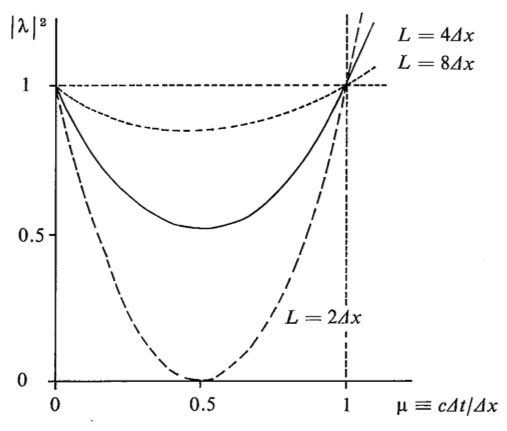
\includegraphics[width = .7 \textwidth]{figs/NM/pic4.jpg}
    \caption{} \label{fig:}
\end{figure}

the graphs of the \(\left| \lambda \right|^{2}\) curves as shown in
\texttt{figg:1}. In general, as the wave length L increases, that is, as
k approaches zero, the amplification factor approaches unity for any
value of the parameter \(\mu\).

The figure shows that within the stable region the scheme is damping for
all values \(\mu \leq 1\). The damping increases as the wave length
decreases. Since the true solution has a constant amplitude, this
damping reveals an error due to finite differencing. We see that this
error increases as the wave length decreases. At the shortest resolvable
wave length, \(L = 2\Delta x\), the error may be very great unless At is
extremely small. It is even possible for this wave to be completely
removed after only a single time step ! The dependence of the error on
wave length, as seen here, might have been anticipated by considering
representation of harmonics of various wave lengths by the finite
difference grid. The shortest resolvable wave, with only two data points
per wave length, is very poorly represented ; as the wave length
increases, the representa­tion by a finite difference grid improves, and
approaches the continuous representation as the wave length tends to
infinity.

There exists a wealth of more precise definitions of stability and
convergence, as well as stability criteria. For a further discussion of
these subjects, and of the relation between the properties of stability
and conver­gence, the interested reader is referred to the book by
Richtmyer and Morton (1967) and to the publication by Kreiss and Oliger
(1973). However, for application of numerical methods to atmospheric
models, it is more important to discuss other problems than to refine
the stability and convergence concepts beyond the outline given here.
These numerical problems, such as phase speed errors and computational
dispersion, nonlinear instability, effect of the space-time grid on the
properties of the numerical solution, and, also the ideas behind and
properties of the great variety of schemes that are currently being used
in atmospheric models, will be discussed in the remaining chapters of
this publication.
